\section{Implementierung}\label{sec:06_04_implementierung}
Die wesentliche Eigenschaft des bereitgestellten Kommunikationsmodells ist, dass es Beziehungen beinhaltet, welche jeweils durch einen Sender, einen Empfänger und eine 
Gewichtung repräsentiert werden. 
Die natürliche Struktur der Daten widerspiegelt ganz offensichtlich diese eines gerichteten Graphs. 
Die Speicherung der Daten in einer Graph-Datenbank ermöglicht die direkte Erkennung von ihren immanenten Beziehungen, was bei tabellenartigen (SQL) oder dokumentenbasierten (NoSQL) Datenbanken ohne komplexe Anfragen deutlich schwieriger ist. 
Die Applikation entspricht also einer ETL\footnote{Extract, Transform, Load}-Pipeline. Sie bezieht sich auf die Erfassung von Daten aus einem externen System und deren Überführung in einem domänenspezifischen
Format, das das Abfragen und die Analyse der Daten erleichtert. 
\begin{figure}[H]
    \centering
    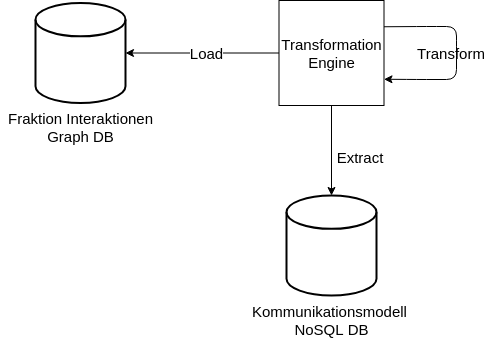
\includegraphics[width=0.60\textwidth]{images/ETL_Factions.png}
    \caption{ETL-Prozess zur Erfassung, Transformation und zum Laden von Daten}
    \label{fig:faction-etl}
\end{figure}
In diesem Fall handelt es sich um die Erfassung von Dokumenten, also Sitzungen des Bundestags, und deren Transformierung in einem gerichteten Graph, dessen Knoten
die Fraktionen der gesamten Legislaturperiode und dessen Kanten die Beziehungen dazwischen sind. Abbildung \ref{fig:faction-etl} stellt eine grobe Architektur dar.  